\documentclass[a4paper, 10pt, final, garamond]{book}
\usepackage{cours-preambule}

\makeatletter
\renewcommand{\@chapapp}{Devoir surveill\'e -- numéro}
\makeatother
% \renewcommand\thechapter{\!\!}

\begin{document}
\setcounter{chapter}{9}

\def\lspace{25}

\chapter{Commentaires sur le DS n\degree\thechapter}
\section{Commentaires généraux}

Bravo pour ce dernier DS~! Les résultats ne sont pas fantastiques, mais en tant
que grosse interrogation c'est pas mal. La partie sur la cristallographie est
assez mal réussie ceci dit, sachant qu'on a fait 2 contrôles dessus \textbf{et}
qu'il n'y a que «~1 seul exercice-type~» de cristallographie. Il faudra
reprendre les techniques de base dessus. Au niveau de l'induction, c'est
passable.

La meilleure note a été placée à 20, ce qui correspond à une moyenne de
\num{10.77}. Le coefficient a été fixé à 1/3 d'un DS.

\begin{center}
	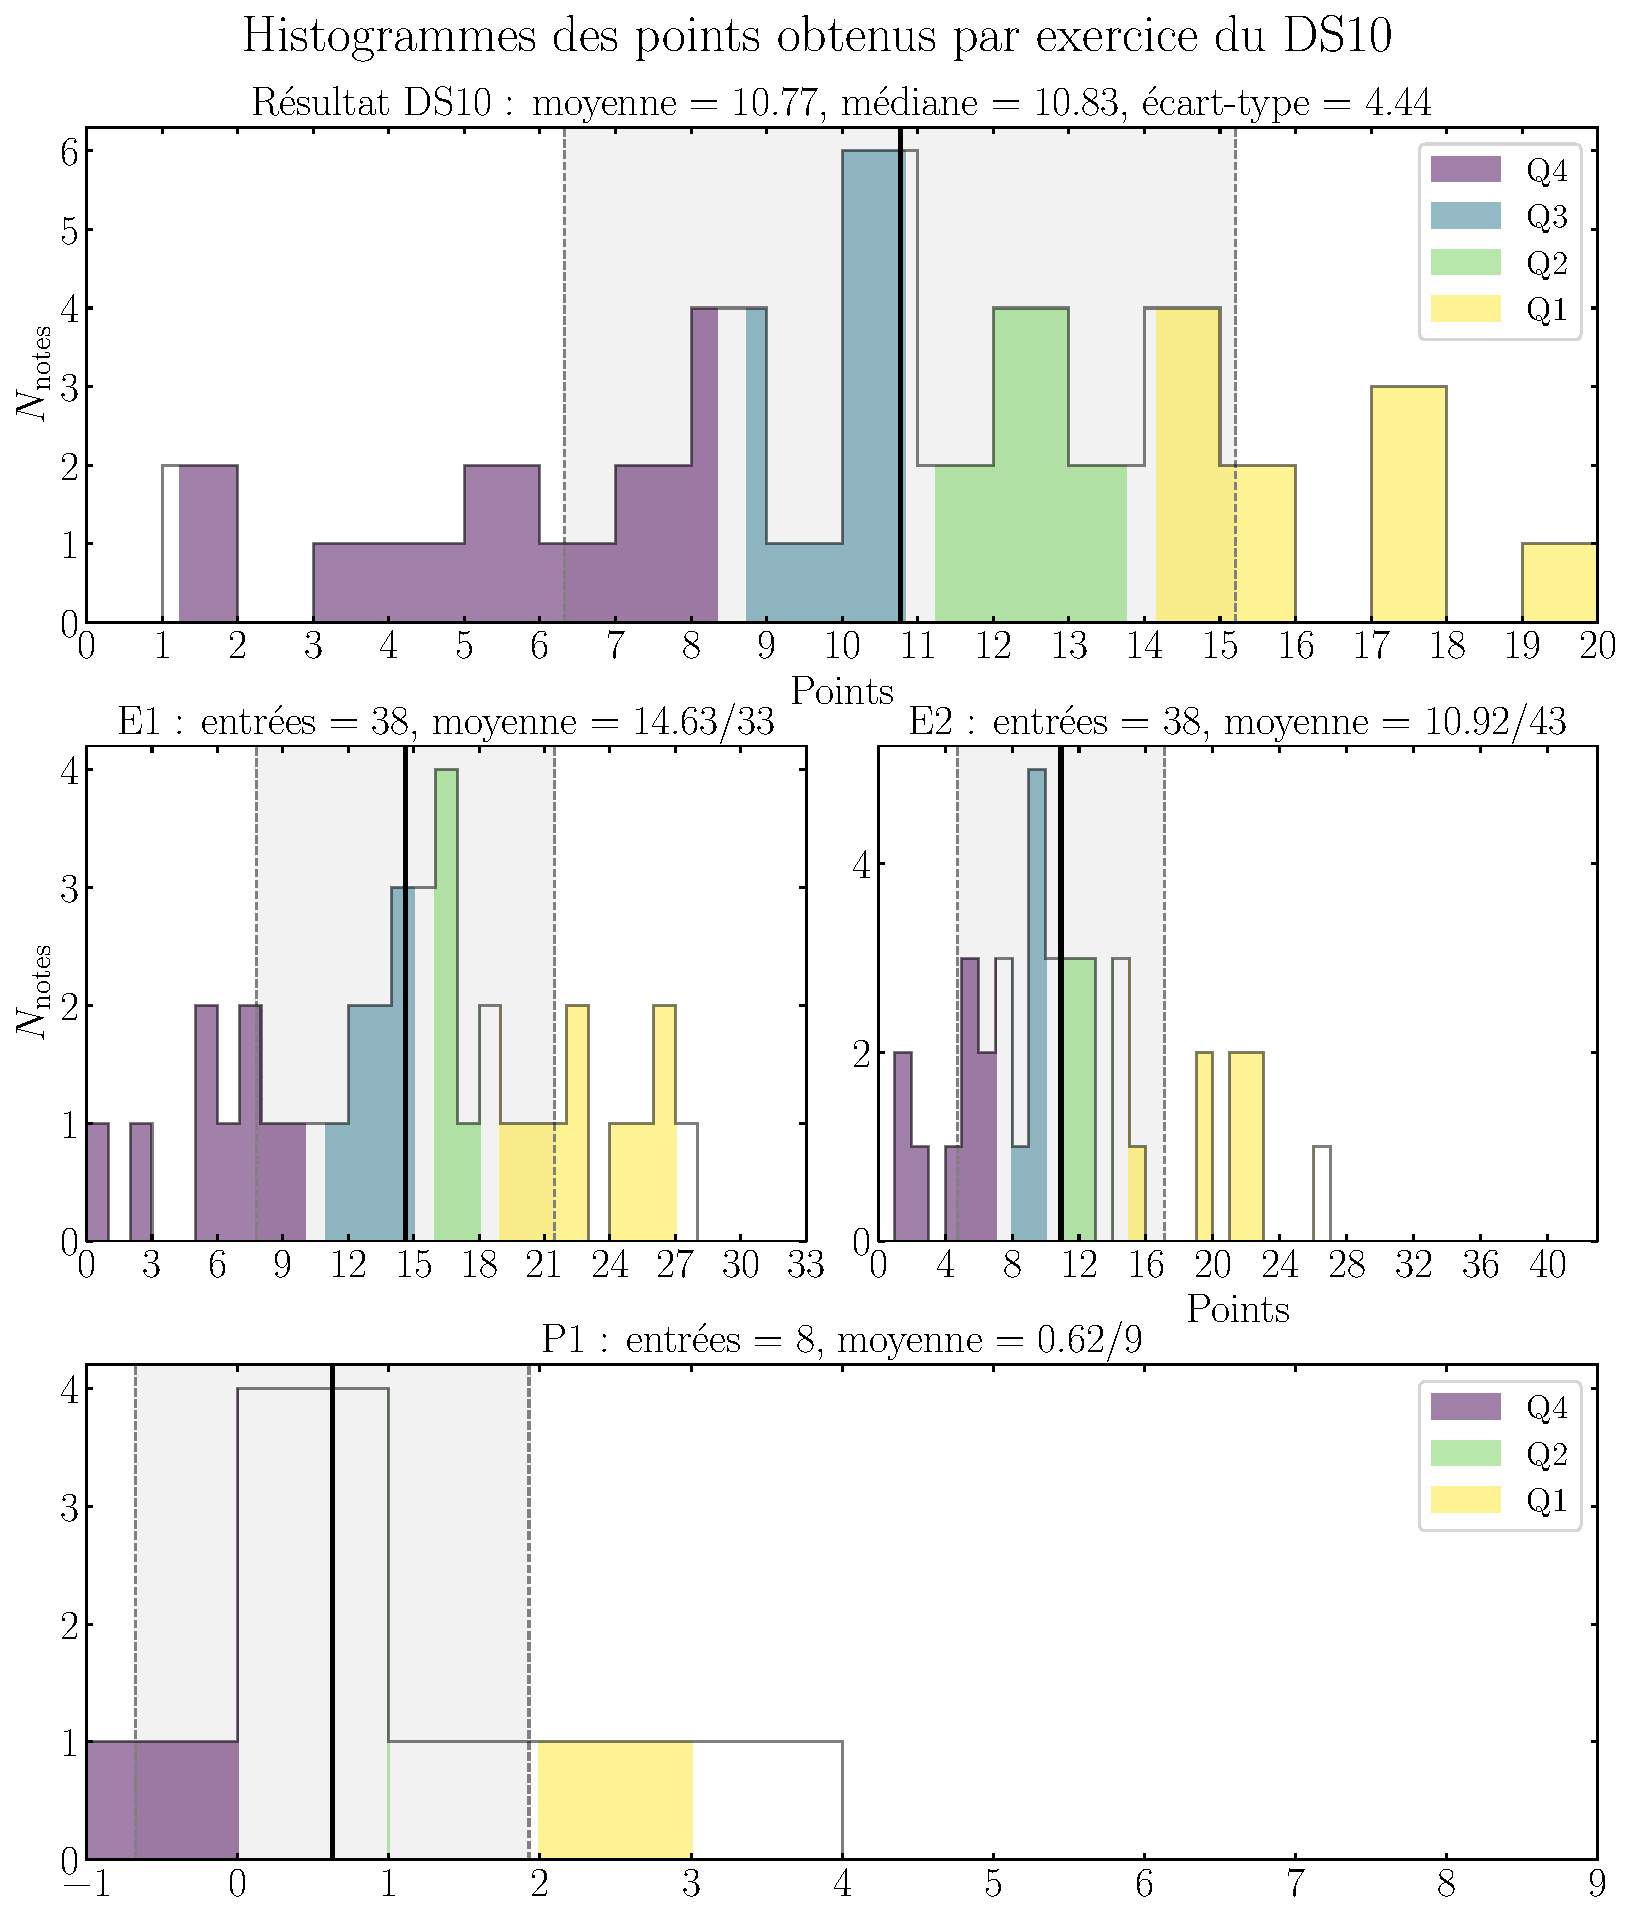
\includegraphics[width=.87\linewidth]{DS10_hist_all}
\end{center}

\setcounter{section}{0}
\section[33]"E"{Étude cristallographique de la chromite}
Trop de confusion sur les définitions. Compacité, coordinence, tangence… il faut
connaître le vocabulaire~!
\begin{enumerate}[label=\sqenumi]
	\item[n]{5} % Q1
	Ici, l'énoncé était sympa, on ne vous demandait de représenter la position
	que d'un seul site de chaque. Il faut retravailler le tracé de la position
	d'un site tétraédrique. Utilisez les grandes diagonales du petit cube par
	exemple.
	\smallbreak
	Il faut cependant que
	votre cube soit bien un cube, et pas un parallélépipède~: les faces doivent
	être carrées~!
	\smallbreak
	Il est interdit de dessiner l'arête «~au fond à gauche~» à la moitié de la
	face de devant~!!
	\smallbreak
	{\Large Achetez une règle~!}
	\item[n]{2} % Q2
	TB.
	\item[n]{4} % Q3
	Il fallait compter \textbf{en propre}~! Il y a 4 sites O en propre…
	\item[n]{3} % Q4
	RAS.
	\item[n]{8} % Q5
	Il \textbf{faut} écrire en toutes lettres où est-ce qu'il y a tangence. Ne
	vous faites pas avoir avec des calculs compliqués~: \textbf{si on vous donne
		$a$ ne vous embêtez pas}. En plus, il fallait interpréter la donnée de
	\textbf{non-tangence} de la maille principale~: on n'a \textbf{pas} $a = 2r
		\sqrt{2}$.
	\item[n]{5} % Q6
	RAS.
	\item[n]{4} % Q7
	La définition n'est pas la formule. De plus, s'il y a plusieurs entités, il
	faut sommer sur les différentes entités.
	\item[n]{2} % Q8
	Idem.
\end{enumerate}

\section[43]"E"{Les phénomènes d'induction -- QCM}
De grosses incohérences, il faudra retravailler ce QCM pour solidifier l'analyse
physique.
\begin{enumerate}[label=\sqenumi]
	\item[n]{4} % Q1
	Manquait de détail, sinon globalement bien. Il faut trouver l'orientation de
	$\vv{S}$.
	\item[n]{6} % Q2
	À revoir. Tous les champs ne sont pas uniformes (c'est même l'inverse), donc
	déplacer un circuit change le flux. Attention, l'énoncé est \textit{un peu}
	traître, on demande ce qui fait varier $B\ind{ext}$. Un courant \textit{dans
		le circuit} ne fait pas varier $B\ind{ext}$~!
	\smallbreak
	Vous ne pouvez pas citer «~l'expérience faite en TP~» sans détailler~!
	\item[n]{2} % Q3
	Même ça… même ça.
	\item[n]{5} % Q4
	Question un peu compliquée mais abordable avec le bon schéma de pensée. Trop
	peu faite ou mal comprise.
	\item[n]{2} % Q5
	Franchement bien~!
	\item[n]{4} % Q6
	À reprendre. Ça n'est pas parce que $M = \frac{\F}{i(t)}$ que $M$ dépend de
	$i$… «~au contraire~» même, puisqu'on a défini que $M$ était la constante
	de proportionnalité entre $\F$ et $i$. Donc $\F$ dépend de $i$~; dire
	«~$\F/i$ dépend de $i$~» n'a pas de sens.
	\item[n]{5} % Q7
	Globalement bien, quand c'est fait.
	\item[n]{2} % Q8
	J'avais fait la remarque de cours sur ce schéma spécifiquement pour cette
	question.
	\item[n]{7} % Q9
	Manquait de détails, et globalement mal faite.
	\smallbreak
	{\Large Force de \textsc{Laplace} $\neq$ induction~!!}
	\item[n]{2} % Q10
	Bien.
	\item[n]{4} % Q11
	Idem, globalement peu clair, manque de détails. \textbf{Attention}, le
	conducteur \textbf{n'est pas aimanté}~!
	\smallbreak
	«~Cf. TP~»~: merci, je sais où trouver l'info… c'est à vous de l'expliquer.
\end{enumerate}

\setcounter{section}{0}
\section[9]"P"{Induction du champ magnétique terrestre dans un téléphone portable}
\begin{enumerate}[label=\sqenumi]
	\item[n]{7} % Q1
	Quelques bons efforts de modélisation~!
	\item[n]{2} % Q2
	Bien essayé pour les réponses qui disent que non, mais sans ordre de
	grandeur des tensions dans un téléphone cette réponse n'est pas recevable.
\end{enumerate}

\end{document}
